% !TeX encoding = UTF-8
\documentclass{vip-theme}

% 中文支持
\usepackage{xeCJK}
\linespread{1.4}

% 全文字体
\setmainfont{Times New Roman}

\title{Learning Scene Structure Guidance via Cross-Task Knowledge Transfer for Single Depth Super-Resolution}
\author{Baoli Sun$^1$, Xinchen Ye$^{1,2*}$, Baopu Li$^3$, Haojie Li$^{1,2}$, Zhihui Wang$^{1,2}$, Rui Xu$^{1,2}$ \\[0.1em]
	$^{1}$International School of Information Science \& Engineering, Dalian University of Technology, China  \\[0.1em]
	$^{2}$Key Laboratory for Ubiquitous Network and Service Software of Liaoning Province, China \\[0.1em]
	$^3$Baidu Research, USA
}

\begin{document}
\begin{sloppypar}
\maketitle
\label{title}

\vspace{0.2em}
\subsection*{Abstract} 
\label{abstract}
Existing color-guided depth super-resolution (DSR) approaches require paired RGB-D data as training samples where the RGB image is used as structural guidance to recover the degraded depth map due to their geometrical similarity. However, the paired data may be limited or expensive to be collected in actual testing environment. Therefore, we explore for the first time to learn the cross-modality knowledge at training stage, where both RGB and depth modalities are available, but test on the target dataset, where only single depth modality exists. Our key idea is to distill the knowledge of scene structural guidance from RGB modality to the single DSR task without changing its network architecture. Specifically, we construct an auxiliary depth estimation (DE) task that takes an RGB image as input to estimate a depth map, and train both DSR task and DE task collaboratively to boost the performance of DSR. Upon this, a cross-task interaction module is proposed to realize bilateral cross task knowledge transfer. First, we design a cross-task distillation scheme that encourages DSR and DE networks to learn from each other in a teacher-student role-exchanging fashion. Then, we advance a structure prediction (SP) task that provides extra structure regularization to help both DSR and DE networks learn more informative structure representations for depth recovery. Extensive experiments demonstrate that our scheme achieves superior performance in comparison with other DSR methods. Our code available at: \href{https://github.com/Sunbaoli/dsr-distillation/}{{\color{vipblue}https://github.com/Sunbaoli/dsr-distillation/}
}.

\section{Motivation}
\label{motivation}


\begin{figure*}[!htbp]
	\centering
	\centerline{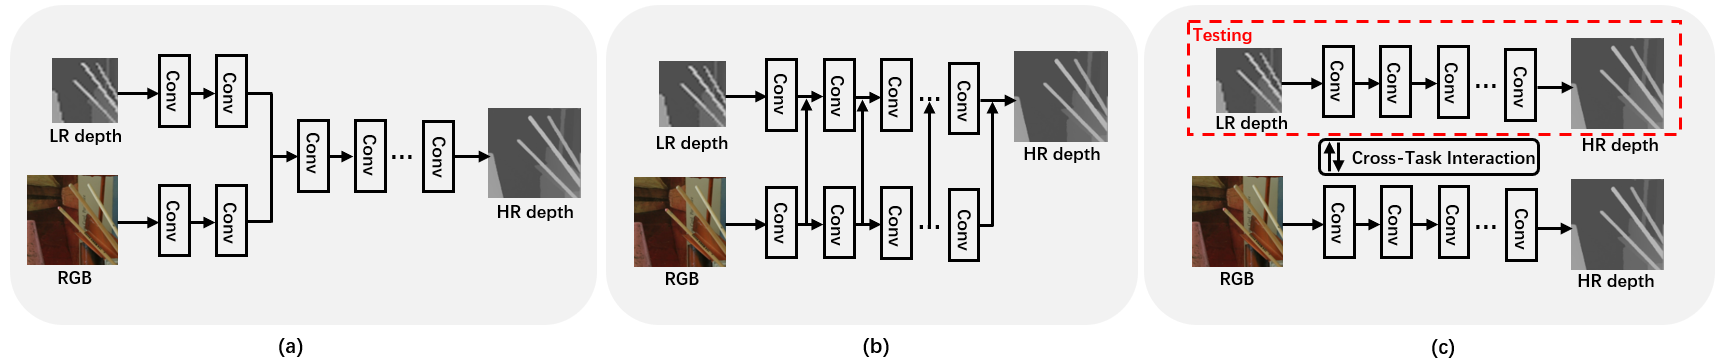
\includegraphics[width=0.97\linewidth]{figure/introduction2.png}}
	\caption{彩色指导深度超分辨率框架:(a)彩色和深度图像联合滤波框架;(b)彩色图像多尺度指导框架;(c)跨任务知识迁移框架}
	\label{fig:intro2}
%\vspace{-4mm}
\end{figure*}
现有的基于颜色图像指导的深度图像超分辨率重建方法,都需要一个额外的分支来从高分辨率彩色图像中提取需要的结构指导信息。但这种模式在实际应用中会受到很多限制。

首先,在实际应用中,与深度图像视角相同且高度配准的高分辨率彩色图像难以直接获取,需要进一步的标定、配准和校正,从而导致了现有训练好的模型无法使用。其次,对于高分辨率彩色图像的处理,极大增加了内存消耗和计算负担,这阻碍了深度图像超分辨率在实际应用中的实时性。此外,高分辨率彩色特征的准确结构信息可以辅助深度图像超分辨率的细节重建,然而,彩色图像的纹理不连续与深度图像的简单结构存在不一致性,彩色图像中同时又包含大量纹理信息,这会导致明显的伪影,如纹理复制和深度泄漏。因此,如何利用有效地利用彩色信息帮助恢复深度图,同时又满足实际测试环境中的实时性要求,还有待进一步探索。

本文希望缓解现有基于彩色指导的深度超分辨率方法的局限性$^1$,\marginpar[1]{\footnotesize $^1$现有的颜色引导的 DSR 方法通过两路融合的架构来利用 RGB-D 图像对,这种架构需要一个额外的分支从 RGB 图像提取结构指导。}如经典的彩色图像与深度图像联合滤波框架$^2$\marginpar{\footnotesize $^2$如图 \ref{fig:intro2}(a)所示,彩色图像和低分辨率深度图像通常由单独的支路处理并通过联合分支“过滤”以输出高分辨率的结果 。但是,由于网络中特定层的特征聚合方式较为简单,来自彩色图像的高频结构信息在特征提取过程中更容易丢失。}和彩色特征多尺度指导框架$^3$\marginpar{\footnotesize $^3$如图 \ref{fig:intro2}(b)所示,一些新颖的方法采用了新的特征聚合范式,即多尺度融合,以允许网络在不同的层级学习丰富的层次特征。这使得网络可以保留更多的空间细节,以便恢复精细结构和大尺度的结构。},从而提出了基于跨任务场景结构知识迁移的单张场景深度图像超分辨率方法,如图 \ref{fig:intro2}(c)所示,为缓解上述问题提供了一个全新的解决思路。




\section{Contribution}
\label{contribution}
本文主要贡献总结如下:
\begin{itemize}
	\item[$\bullet$] 本文提出的 DSR 范式是第一个在训练阶段以多种模态作为输入进行学习,但仅在单个 LR 深度模态上进行测试的工作。本文提出的基于跨任务场景结构知识迁移的单张深度图像超分辨率框架,在训练阶阶段构建了一个以彩色图像为输入的深度估计任务,以及以低分辨率深度图像为输入的深度超分辨率任务,并对两个任务进行协同训练;

	\item[$\bullet$] 提出了一个跨任务知识交互模块从彩色图像中蒸馏需要的结构信息辅助深度图像的恢复,以鼓励 DSRNet 和 DENet 在协作训练模式下相互学习;

	\item[$\bullet$] 提出了多空间知识蒸馏策略以及不确定度引导的结构正则化约束来实现双边知识迁移,提升深度超分辨率模型的性
能。

\end{itemize}

\section{Method}
\label{method}
\subsection{基于跨任务场景结构知识迁移的单张深度图像超分辨率网络}

图 \ref{fig:mainnet} 展示了基于跨任务场景结构知识迁移的单张深度图像超分辨率的框架,主要由深度超分辨率网络(DSRNet)、深度估计网络(DENet)和中间跨任务交互模块(CT)三部分组成。给定一组配对的 LR-HR 深度图像 $\left\{D_{l r}^{(k)}, D_{h r}^{(k)}\right\}_{k=1}^{M}$ 以及对应的 HR 彩色图像 $\{I(k)\}_{k=1}^{M}$ 作为训练数据,其中 $M$ 为训练数据的个数,最终的目标是训练 DSRNet 使其能够从单张 LR 深度图像 $\left\{D_{l r}^{(k)}\right\}_{k=1}^{M}$ 得到超分结果 $\left\{D_{s r}^{(k)}\right\}_{k=1}^{M}$。

DSRNet 的结构是基于 deep back-projection network (DBPN) 的网络单元设计的,如图 \ref{fig:mainnet} 红框所示,该网络通过将 HR 表示迭代投影到 LR 空间域,再映射回 HR 域,有效地增强了特征表示。首先通过三个简单的卷积层对 $D_{lr}$ 提取特征得到 $D_{sr}^{shallow}$,然后将 $D_{sr}^{shallow}$ 送入主干网络获得 HR 特征 $\{F_{sr}^n\}_{n=1}^N$,$N$ 是堆叠的 DBPN 模块的数量。最后将 $F_{sr}^N$ 通过一个简单的卷积块映射到输出空间。得到超分辨率网络的输出 $D_{sr}$。

DENet 的结构与 DSRNet 类似,但是用了更深的残差块代替 DBPN 块从彩色图像中提取特征 $\{F_{de}^n\}_{n=1}^N$。最后将 $F_{de}^N$ 通过一个简单的卷积块映射到输出空间。得到深度估计网络的输出 $D_{de}$。

\begin{figure*}[!htbp]
	\centering
	\centerline{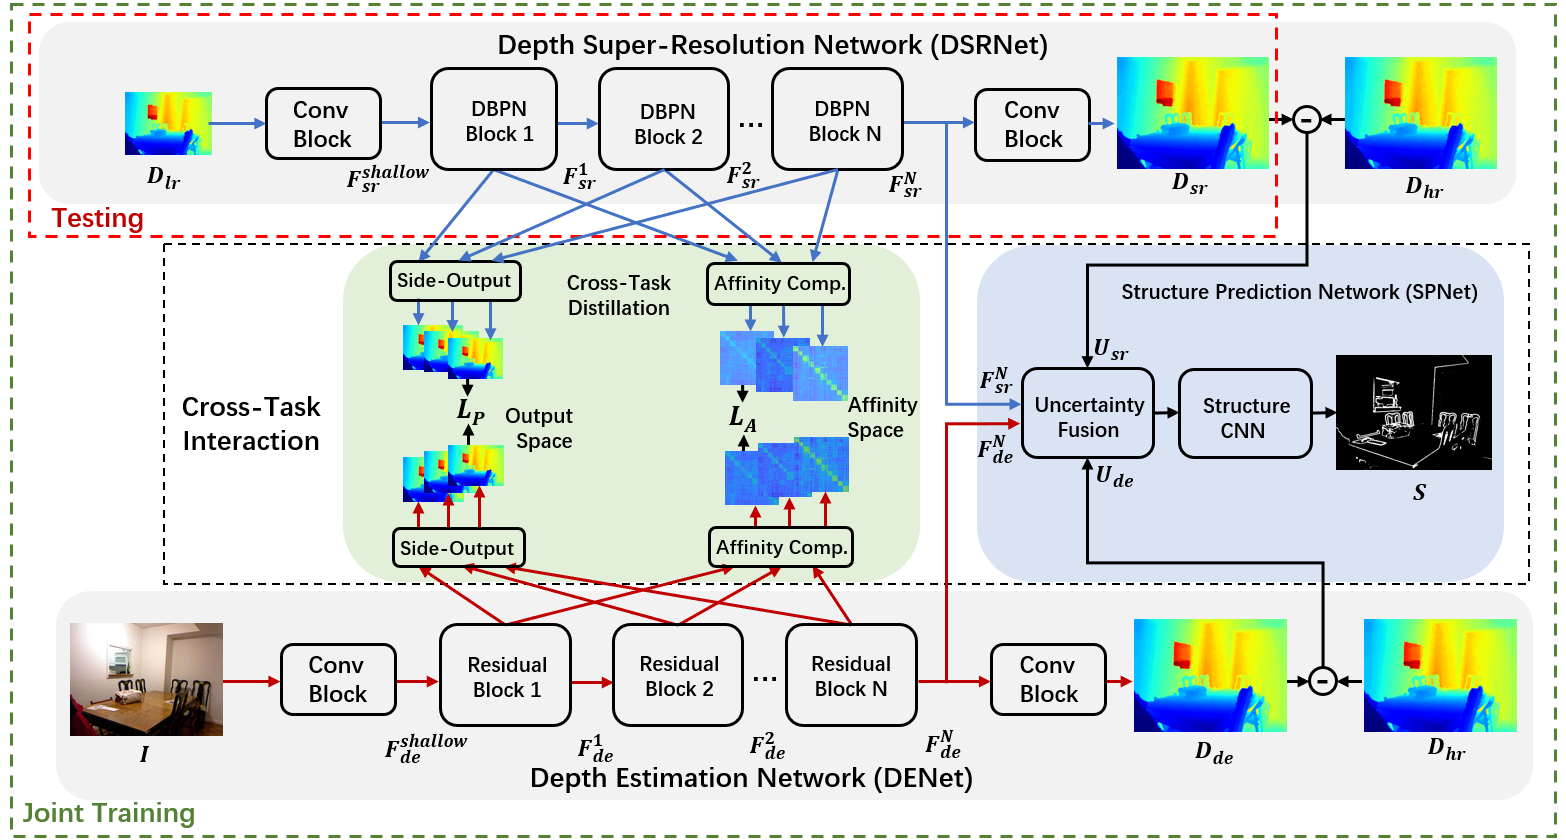
\includegraphics[width=1\linewidth]{figure/mainnet8.png}}
	\caption{基于跨任务场景结构知识迁移的单张深度图像超分辨率网络, 由 DSRNet、DENet 和中间的跨任务交互模块组成。该网络使用相同的真实深度图像 $D_{hr}$ 监督 DSRNet 和 DENet 的输出。在测试阶段,DSRNet 是不借助彩色图像仅从 LR 深度图像预测 HR 深度图像的最终选择。}
	\label{fig:mainnet}
\vspace{-4mm}
\end{figure*}

CT 是连接 DSRNet 和 DENet 的桥梁,实现了 DSRNet 和 DENet 之间的双边知识转移。CT 由两部分组成,即跨任务知识蒸馏(Cross-Task Distillation)和结构预测网络(Structure Prediction Network,SPNet),前者侧重于从两个网络中提取的多尺度特征之间的交互,而后者则使用结构图作为监督,进一步指导两个网络的学习。

\subsection{跨任务知识蒸馏策略}

知识蒸馏通常被认为是一种将有益的信息从一个性能最佳的模型转移到另一个简单模型的技术,其教师网络提前训练然后固定参数,而且假设它总是比学生网络能够学习更好的表示。不同于常用的蒸馏技术,本文的目标是协作训练 SRNet 和 DENet 并鼓励他们互相受益。

在相互学习(Mutual Learning)方法的启发下,本文提出了一种跨任务知识蒸馏方案,根据迭代的协作训练中老师和学生网络在深度恢复方面的当前表现,在两个任务之间进行师生角色切换。特别的,在当前这轮训练中,需要根据它们上一轮的表现提前确定老师。计算每个恢复深度图和对应真实深度图像之间的平均像素误差:

\begin{equation}\label{esr}
e_{dsr} = \frac{1}{HW}\sum_h^H\sum_w^W|D_{sr}(h,w) -D_{hr}(h,w)|,
\end{equation}
\begin{equation}\label{ede}
e_{de} = \frac{1}{HW}\sum_h^H\sum_w^W|D_{de}(h,w) -D_{hr}(h,w)|,
\end{equation}

式中 $\{H,W\}$ 为输出深度图像的大小。$e_{dsr}$ 小于 $e_{de}$ 时,DSRNet 的性能相对较好,成为引导 DENet 学习的老师网络,反之,$e_{de}$ 小于 $e_{dsr}$ 时,DENet 的性能相对较好,成为引导 DSRNet 学习的老师网络。

为了可以蒸馏出更有意义的、能够准确表达深度图像本质结构特征的知识,本文提出了一种多空间蒸馏策略,在输出空间和结构空间对知识进行迁移。

\begin{enumerate}
	\item[(1)] \textbf{输出空间蒸馏(Output Space Distillation)} :为了确保深度图像中像素级深度值的局部信息传输,本章在 DSRNet 和 DENet 的中间加入了边界输出层(包含两个简单的卷积层)将两个网络的多级特征 $\left\{F_{s r}^{n}, F_{d e}^{n}\right\}_{n=1}^{N}$ 映射到输出空间。因此,输出空间蒸馏的损失函数被设计成间接对齐 DSRNet 和 DENet 之间的特征:
	
	\begin{equation}
\mathcal{L}_{O}=\frac{1}{N} \sum_{n=1}^{N}\left\|D_{s r}^{n}-D_{d e}^{n}\right\|_{1}
\end{equation}

\item[(2)] \textbf{结构空间蒸馏(Affinity Space Distillation)}:彩色图像及其对应深度图像是对同一场景的不同表示,具有很强的结构相似性。在彩色图像中,外观相似的像素有更多的机会属于同一个对象,并且应该有接近的深度值。一些探索像素间相关性的工作考虑非局部相关来增强像素之间的相关特征,有利于深度图像恢复。本文也将非局部结构知识转移到结构空间,通过计算像素对之间的相似性来实现。

假设特征图 $F$ 的维度为 $h \times w \times c$,变形函数 $\mathbb{R}$ 的功能就是改变 $F$ 的维度为  $hw \times c$,相似度矩阵定义为:

\begin{equation}
A(F)=\sigma\left(\mathbb{R}(F) \otimes \mathbb{R}^{T}(F)\right)
\end{equation}

其中,$\sigma(\cdot)$ 是 Softmax 激活函数,$\otimes$ 代表矩阵乘法,$T$ 是矩阵转置操作。所以结构空间蒸馏的损失函数定义为对齐 DSRNet 与 DENet 多级特征的相似度矩阵:

\begin{equation}
\mathcal{L}_{A}=\frac{1}{N} \sum_{n=1}^{N}\left\|A\left(F_{S r}^{n}\right)-A\left(F_{d e}^{n}\right)\right\|_{1}
\end{equation}

整体的蒸馏损失函数为输出空间蒸馏损失与特征空间蒸馏损失的和:

\begin{equation}
\mathcal{L}_{\text {distill }}=\mathcal{L}_{O}+\gamma \mathcal{L}_{A}
\end{equation}

其中,$\gamma$ 是一个平衡参数。$\mathcal{L}_{\text {distill }}$ 应该用于对学生网络的更新,而不是对老师网络的更新,这是由 $e_{dsr}$ 和 $e_{de}$ 之间的大小决定的。

\end{enumerate}

\subsection{结构预测子网络}	

\begin{figure*}
	\centering
	\centerline{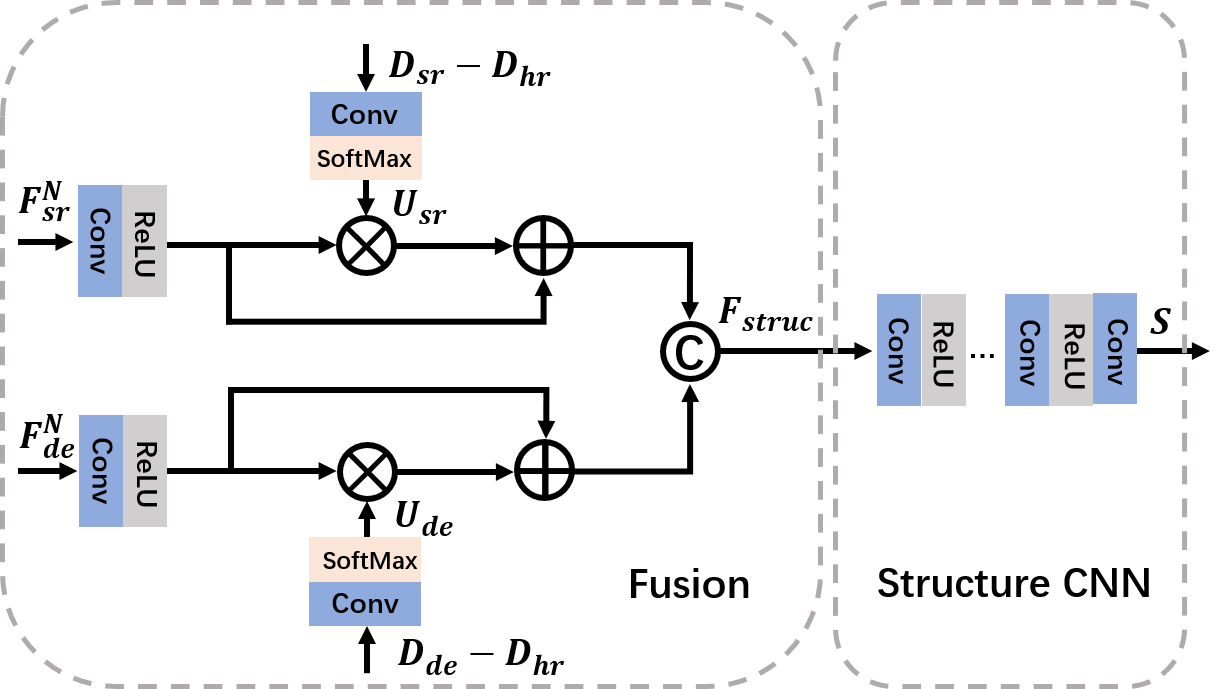
\includegraphics[width=0.65\linewidth]{figure/gradient_block4.png}}
	\caption{结构预测子网络}
	\label{fig:block}
\end{figure*}

结构预测网络(Structure Prediction Net,SPNet)的目标是根据 DSRNet 和 DENet 的特征图 $F_{sr}^N$ 和 $F_{de}^N$ 预测一个结构图 $S$,提供额外的结构正规化,帮助 DSRNet 和 DENet 学习更多的信息结构表示,缓解 RGB-D 结构不一致的问题。SPNet 通过由真实结构图 $S_{gt}$,$S_{gt}$ 通过计算真实高分辨率深度图像 $D_{hr}$ 中相邻像素的差值(梯度)得到。如图 \ref{fig:block} 所示,所示,SPNet 由一个融合模块和一个结构预测 CNN 组成,融合模块对 DSRNet 和 DENet 的特征图 $F_{sr}^N$ 和 $F_{de}^N$ 进行融合,结构 CNN 是一个轻量级网络,包含五个堆叠的卷积层,将融合后的特征映射到输出空间。通常 DSR 和 DE 任务的错误恢复通常发生在深度图像中的深度边界和精细结构附近的区域,具有较高的恢复不确定性。因此,本文不是简单地将 $F_{sr}^N$ 和 $F_{de}^N$ 连接起来送入到结构 CNN 中,而是设计一个不确定性诱导的注意力融合模块,通过将恢复的不确定性加入到特征图中来加强这些结构特征。因此,首先通过激活重建误差图来计算两个网络的不确定度 $U_{sr}$ 和 $U_{de}$:
 
\begin{equation}
\begin{aligned}
&U_{s r}=\sigma\left(\operatorname{Conv}_{1 \times 1}\left(D_{s r}-D_{h r}\right)\right. \\
&U_{d e}=\sigma\left(\operatorname{Conv}_{1 \times 1}\left(D_{d e}-D_{h r}\right)\right.
\end{aligned}
\end{equation}

其中,$Conv_{1 \ times 1}$ 是一个卷积核大小为 $1 \times 1$ 的卷积层,作用是调整通道数。然后,使用不确定性映射重新对  $F_{sr}^N$ 和 $F_{de}^N$ 赋予权重并通过注意模块将其融合。

\begin{equation}
F_{\text {struct }}=\left[F_{s r}^{N} *\left(1+U_{s r}\right), F_{d e}^{N} *\left(1+U_{d e}\right)\right]
\end{equation}

其中, $F_{\text {struct}}$ 是融合后的特征,$[\cdot]$ 表示串联操作,$*$ 表示像素级的乘法。通过从 SPNet在逆向信息流中反向传播的梯度,可以更新 DSRNet 和 DENet 的参数。

\subsection{训练策略}
 
整体的基于跨任务场景结构知识迁移的单张深度图像超分辨率网络的训练过程可以分为两个步骤,如算法 \ref{algorithm} 所示。
 
\textbf{第一阶段}:首先用真实深度图像 $D_{hr}$ 训练 DSRNet 和 DENet。损失的定义如下:

\begin{equation}
\begin{gathered}
\mathcal{L}_{D S R}=\left\|D_{s r}-D_{h r}\right\|_{1} \\
\mathcal{L}_{D E}=\lambda \frac{1-\operatorname{SSIM}\left(D_{d e}, D_{h r}\right)}{2}+(1-\lambda)\left\|D_{d e}-D_{h r}\right\|_{1}
\end{gathered}
\end{equation}
,
其中,$L_{DSR}$ 是常见的像素级的 L1 损失函数用于监督 DSRNet 的学习,$L_{DE}$ 被定义为重建 L1 损失函数和结构相似度损失函数的和,$\lambda$ 是一个平衡参数。

\textbf{第二阶段},在两个网络之间引入跨任务蒸馏损失函数 $\mathcal{L}_{\text {distill }}$,同时引入 SPNet,SPNet 和 DSRNet 与 DENet 同时训练。SPNet 的损失函数定义为:

\begin{equation}
\mathcal{L}_{D S R}=\left\|\mathbb{G}\left(F_{\text {struc }}\right)-S_{g t}\right\|_{1}
\end{equation}

其中,$\mathbb{G}$ 表示 SPNet,$F_{\text {struct}}$ 为融合的特征。如果 DSRNet 被判定为学生,则 DENet 的参数在当前是固定的,DSRNet 将按照下面的损失函数进行更新:

\begin{equation}
\mathcal{L}=\mathcal{L}_{D S R}+\rho_{1} \mathcal{L}_{\text {struc }}+\rho_{2} \mathcal{L}_{\text {distill }}
\end{equation}

其中,$\rho_1$ 和 $\rho_2$ 为平衡参数。当 DENet 被判定为学生,则 DSRNet 的参数在当前是固定的,DENet 将按照下面的损失函数进行更新:

\begin{equation}
\mathcal{L}=\mathcal{L}_{D E}+\rho_{1} \mathcal{L}_{\text {struc }}+\rho_{2} \mathcal{L}_{\text {distill }}
\end{equation}




\vspace{2em}
\begin{algorithm}[H]
        \caption{Training Details}
        \label{algorithm}
        \LinesNumbered
        \KwIn{Training data {$D_{lr}$, $D_{hr}$, $I$,  $S_{gt}$} %three networks $W_{SR}$, $W_{DE}$ and $W_{GE}$ \\Initialise $W_{SR}$, $W_{DE}$ and $W_{GE}$
        }
        \KwOut{$D_{sr}$}
        ---------------- Step 1 ----------------\\
        Randomly initialize DSRNet and DENet\\
       
        \For {i = 1; i $\leq$ 100;}
        {
%         ——————————————— Step 1 ———————————————\\
         Train DSRNet and DENet with $\mathcal{L}_{DSR}$ and $\mathcal{L}_{DE}$, respectively\\
         }
         ---------------- Step 2 ----------------\\
         Randomly initialize SPNet\\
         \For {i = 101; i $\le$ max epoch}
         {
         Compute the average error value $e_{dsr}$ and $e_{de}$ according to Eq.(\ref{esr}) and Eq.(\ref{ede})\\
         \If {$e_{dsr} \le e_{de}$}
         {
        Fix DSRNet and update DENet with $\mathcal{L} = \mathcal{L}_{DE} + \rho_1\mathcal{L}_{struc} + \rho_2\mathcal{L}_{distill}$
        }
        \Else
        {
        Fix  DENet and update DSRNet with $\mathcal{L} = \mathcal{L}_{DSR} + \rho_1\mathcal{L}_{struc} + \rho_2\mathcal{L}_{distill}$
         }
         }
  
    \end{algorithm}

%\begin{algorithm}[!t]
%	\caption{Training Details}
%	\label{algorithm11}
%	\begin{algorithmic}[1]
%		
%		\Require Training data {$D_{lr}$, $D_{hr}$, $I$,  $S_{gt}$} %three networks $W_{SR}$, $W_{DE}$ and $W_{GE}$ \\Initialise $W_{SR}$, $W_{DE}$ and $W_{GE}$
%        \State ---------------- Step 1 ----------------
%        \State Randomly initialize DSRNet and DENet
%        \For {i = 1; i $\le$ 100}
%        \State Train DSRNet and DENet with $\mathcal{L}_{DSR}$ and $\mathcal{L}_{DE}$, respectively
%		\EndFor
%        \State ---------------- Step 2 ----------------
%		%\State Initialize whole network with random weights, train the SR-Net and DE-Net respectively
%        \State Randomly initialize SPNet
%		\For {i = 101; i $\le$ max epoch}
%        \State Compute the average error value $e_{dsr}$ and $e_{de}$ according to Eq.(\ref{esr}) and Eq.(\ref{ede})
%        \If {$e_{dsr} \le e_{de}$}
%        \State Fix DSRNet and update DENet with
%		\State $\mathcal{L} = \mathcal{L}_{DE} + \rho_1\mathcal{L}_{struc} + \rho_2\mathcal{L}_{distill}$
%        \Else
%        \State Fix  DENet and update DSRNet with
%        \State $\mathcal{L} = \mathcal{L}_{DSR} + \rho_1\mathcal{L}_{struc} + \rho_2\mathcal{L}_{distill}$
%        \EndIf
%		\EndFor
%        \Ensure $D_{sr}$
%			
%	\end{algorithmic}
%\end{algorithm}

\section{Experiments}
\label{experiments}

以 MIDDLEBURY 数据集为例,首先在四个常见倍率($2\times$、$4\times$、$8\times$ 和 $16\times$)的超分辨率任务上对比了多个最先进的深度图像超分辨率方法,如表 \ref{table:compar} 所示。得益于 DBPN 骨干网络,DSRNet w/o CT 的性能超过了以前的大多数方法,但略低于最近的先进的方法。


\begin{table*}[!htbp]
	\begin{center}
		\caption{在 Middlebury 2005 数据集上 $8 \times$ 的性能比较。 `DSRNet w/o CT' 和 `DSRNet' 分别表示所提出方法没有和有跨任务交互方案的的结果。}
		 \fontsize{8.0}{13}\selectfont
		\label{table:compar}
		\scalebox{0.6}{
			\begin{tabular}{c|cccc|cccc|cccc|cccc|cccc|cccc}				
				\toprule
				\multirow{2}[3]{*}{} & \multicolumn{4}{c}{\textit{Art}} & \multicolumn{4}{c}{\textit{Books}} & \multicolumn{4}{c}{\textit{Dolls}} & \multicolumn{4}{c}{\textit{Laundry}} & \multicolumn{4}{c}{\textit{Moebius}} & \multicolumn{4}{c}{\textit{Reindeer}}\\			\cmidrule{2-25}&$\times$2&$\times$4&$\times$8&$\times$16&$\times$2&$\times$4&$\times$8&$\times$16&$\times$2&$\times$4&$\times$8&$\times$16&$\times$2&$\times$4&$\times$8&$\times$16&$\times$2&$\times$4&$\times$8&$\times$16 &$\times$2&$\times$4&$\times$8&$\times$16 \\\hline
				Bicubic & 0.48  & 0.97  & 1.85  & 3.59  & 0.13  & 0.29  & 0.59  & 1.15  & 0.20   & 0.36  & 0.66  & 1.18 & 0.28  & 0.54  & 1.04  & 1.95  & 0.13  & 0.30   & 0.59  & 1.13  & 0.30   & 0.55  & 0.99  & 1.88\\
				DJF & 0.12  & 0.40   & 1.07  & 2.78  & 0.05  & 0.16  & 0.45  & 1.00     & \textbf{0.06}  & 0.20   & 0.49  & 0.99  & 0.07  & 0.28  & 0.71  & 1.67  & 0.06  & 0.18  & 0.46  & 1.02  & 0.07  & 0.23  & 0.60   & 1.36\\
				
				MSG & \quad-  & 0.46  & 0.76  & 1.53  & \quad-  & 0.15  & 0.41  & 0.76  & \quad-  & 0.25  & 0.51  & 0.87 &  \quad-     & 0.30   & 0.46  & 1.12  & \quad-  & 0.21  & 0.43  & 0.76  & \quad-  & 0.31  & 0.52  & 0.99\\
				DGDIE & 0.20   & 0.48  & 1.20   & 2.44  & 0.14  & 0.30   & 0.58  & 1.02  & 0.16  & 0.34  & 0.63  & 0.93 & 0.15  & 0.35  & 0.86  & 1.56  & 0.14  & 0.28  & 0.58  & 0.98  & 0.16  & 0.35  & 0.73  & 1.29\\
				DEIN &0.23   &0.40   &0.64   &\textbf{1.34}  &0.12   &0.22   &0.37   &0.78   &0.12   &0.22   &0.38   &0.73  &0.13   &0.23   &0.36   &0.81   &0.11   &0.20   &0.35  &0.73   &0.15   &0.26   &0.40  & 0.80 \\				
                CCFN & \quad-  & 0.43  & 0.72  & 1.50   & \quad-  & 0.17  & 0.36  & 0.69  & \quad-  & 0.25  & 0.46  & 0.75 &   \quad-    & 0.24  & 0.41  & \textbf{0.71}  & \quad-  & 0.23  & 0.39  & 0.73  & \quad-  & 0.29  & 0.46  & 0.95\\
                GSRPT &0.22 &0.48 &0.74 &1.48&0.11 &0.21  & 0.38  &0.76&0.13 &0.28  & 0.48 & 0.79&0.12 &0.33  & 0.56  &1.24&0.12 & 0.24  &0.49  &0.80
                &0.14 & 0.31  &0.61  &1.07 \\
               DSRN &0.12   &0.25   &0.61   &1.80  &\textbf{0.04}   &\textbf{0.11}  &0.28   &0.69   &\textbf{0.06}   &\textbf{0.14}  &\textbf{0.33}   &0.73  &\textbf{0.06}   &\textbf{0.15}   &0.43   &1.24  &\textbf{0.05}   &\textbf{0.13}  &0.29  &\textbf{0.67}   &\textbf{0.07}   &\textbf{0.15}   &\textbf{0.35}  & 0.92 \\ \hline
               DSRNet w/o CT &0.16 &0.31 & 0.59&1.55 & 0.10& 0.15&  0.31 &0.73 &0.12 & 0.21& 0.39 &0.69 &0.12 & 0.21& 0.40  &0.82 & 0.11& 0.16& 0.32 &0.74 & 0.13&  0.22& 0.38 &0.87\\
				DSRNet & \textbf{0.11} & \textbf{0.25} & \textbf{0.53}& 1.44 & 0.05 & \textbf{0.11} & \textbf{0.26} & \textbf{0.67} &  0.07 & 0.16 & 0.36 & \textbf{0.65} & \textbf{0.06} & 0.16 & \textbf{0.36}  & 0.76 & 0.07 & \textbf{0.13} & \textbf{0.27} & 0.69 & 0.08 & 0.17 & \textbf{0.35} & \textbf{0.77} \\
				\bottomrule				
		   \end{tabular}}
	\end{center}
\vspace{-4mm}
\end{table*}

\begin{figure*}[!htbp]
	\centering
	\centerline{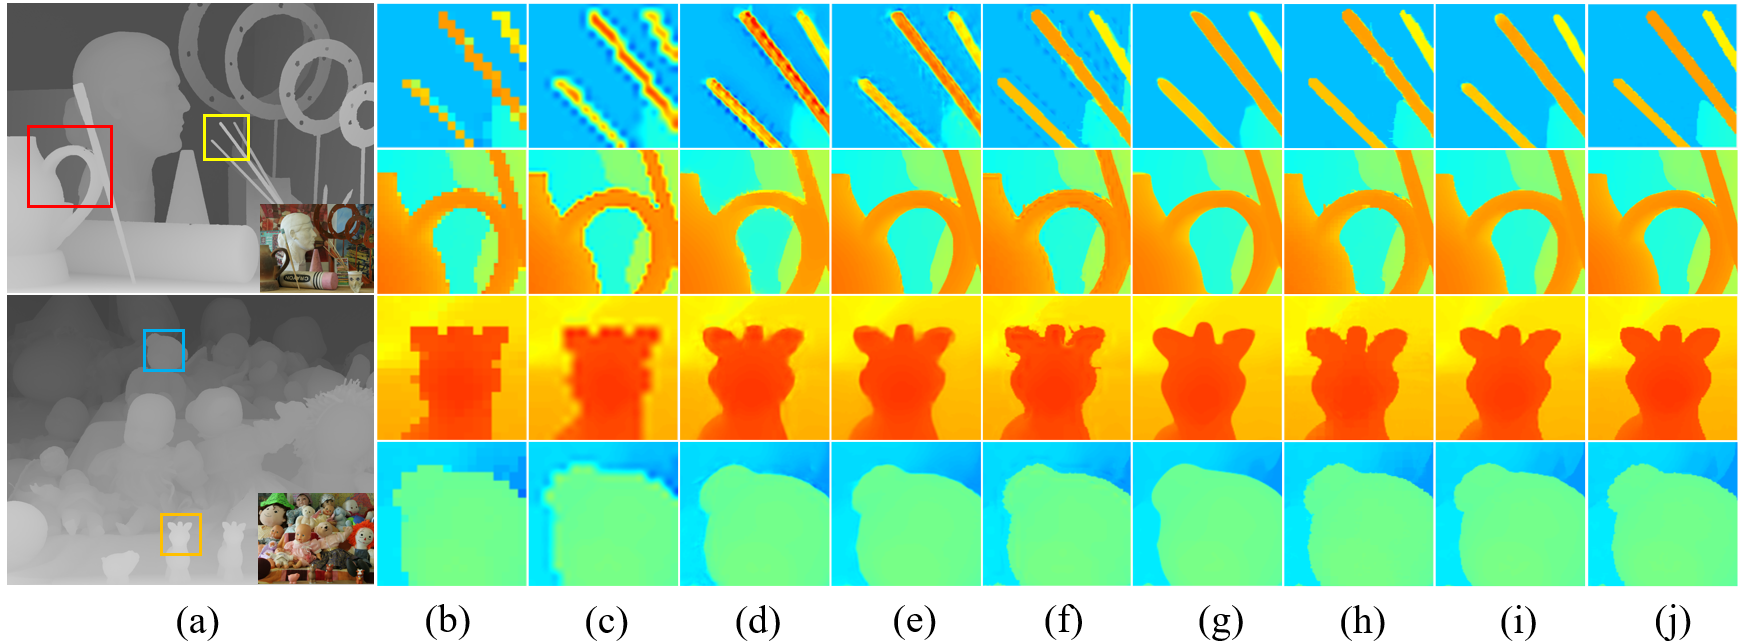
\includegraphics[width=1\linewidth]{figure/compar.png}}
	\caption{在 Middlebury 2005 数据集上 $8 \times$ 的结果比较。(a)GT depth maps;(b)LR;(c)
Bicubic;(d)DJF;(e)DGDIE;(f)DEIN;(g)GSRPT;(h)DSRN;(i)Ours;(j)GT。}
	\label{fig:compar}
\end{figure*}
%\newpage

当与 DENet 一起进行跨任务交互的的协同训练时,本文的 DSRNet 的性能比不带 CT 时的 DSRNet 更进一步,与 DSRN 性能相当,甚至在至少一半的测试样本中比 DSRN 性能更好。需要强调的是,与这些色彩指导的 DSR 方法不同,在测试阶段仅使用单张 LR 深度图像作为网络输入,没有 HR 彩色图像的帮助,但在准确性和运行时间都取得了令人满意的结果。如图 \ref{fig:compar} 所示,展示了 $8 \times$ DSR 的主观结果。对于结构细节,如第一个测试样本中的棍子和茶壶柄,第二张测试样本中的玩具轮廓,本文的基于场景结构的跨任务迁移框架,在不引入纹理模糊的情况下,清晰地恢复了这些区域。

在图 \ref{fig:run_time} 中,通过精确度和运行时之间的权衡总结了总体性能。在Middlebury 数据集上,在完全分辨率约 $1080 \times 1320$ 的测试样例上测试了 $8 \times$ DSR 的运行时间和准确度。由于在测试阶段使用了 HR 彩色图像,彩色指导方法即 JGF,MSG 和 DSRN 比本章的方法运行得慢。MS 是 MSG 的单张深度图 DSR 版本,但在准确性和速度上仍然不如本章的方法。由于任务间的交互作用,本章的方法以最小的推理时间获得了满意的恢复结果。

\begin{figure*}[!htbp]
	\centering
	\centerline{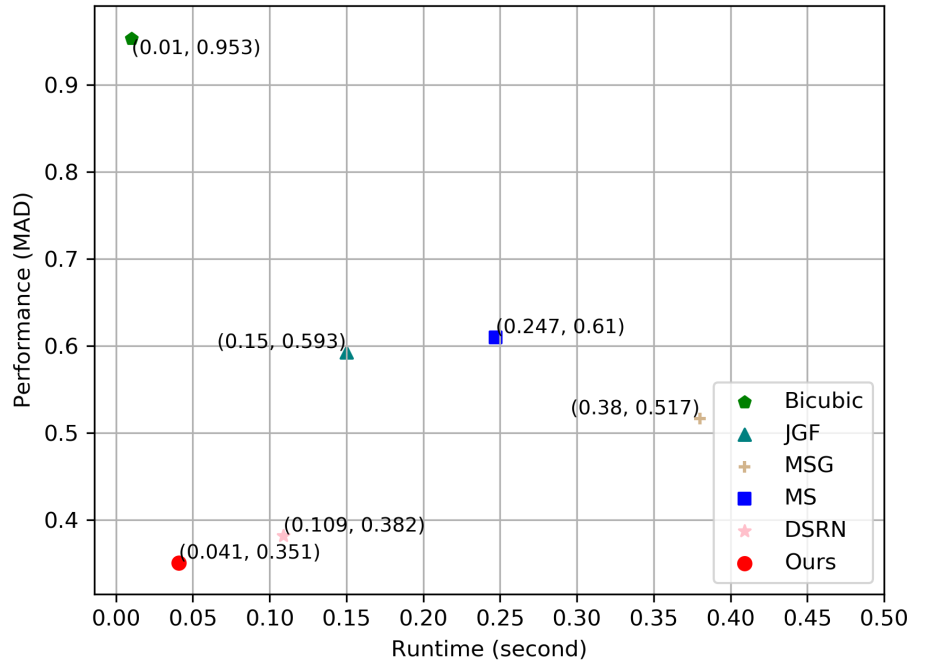
\includegraphics[width=0.95\linewidth]{figure/run_time.png}}
	\caption{运行时间与性能}
	\label{fig:run_time}
\end{figure*}

\end{sloppypar}
\end{document}